\documentclass[10pt]{article}
\usepackage[a4paper, margin=1in]{geometry}
\usepackage[utf8]{inputenc}
\usepackage[spanish]{babel}
\usepackage{caratula}
\usepackage{amsmath}
\usepackage{amssymb}
\usepackage{hyperref}
\usepackage{enumitem}
\usepackage{graphicx}
\usepackage{subcaption} % Para subfiguras
\usepackage{xcolor}

\hypersetup{
    colorlinks=true,
    linkcolor=blue,
    filecolor=magenta,      
    urlcolor=cyan,
    pdftitle={Overleaf Example},
    pdfpagemode=FullScreen,
	}
	
\setlength{\parskip}{1em}   % Espacio vertical entre párrafos

\begin{document}

	\titulo{TP3}

	\fecha{\today}

	\materia{Introducción a la Investigación Operativa y Optimización}

	\integrante{Laks, Joaquín}{425/22}{laksjoaquin@gmail.com}
	\integrante{Szabo, Jorge}{1683/21}{jorgecszabo@gmail.com}
	\integrante{Wilders Azara, Santiago}{350/19}{santiago199913@gmail.com}

	\maketitle

\section{Introducción}

En este trabajo práctico se implementaron distintos algoritmos para encontrar la ubicación óptima de un centro de servicio médico que responda a zonas afectadas con distintos niveles de atención necesarios. Se busca encontrar un punto que minimice la suma de las distancias euclidianas ponderadas respecto a un conjunto discreto de puntos, es decir, encontrar la mediana geométrica de dicho conjunto.

Formalmente, dado un conjunto de puntos $ \mathbf{P} = \{p_1, \dots, p_m\} \subset \mathbb{R}^n$ y pesos $w_1, \dots, w_m > 0$, el problema se reduce a encontrar:
\[
\mathbf{x}^* = \arg \min_{\mathbf{x} \in \mathbb{R}^n} W(\mathbf{x}) = \sum_{i=1}^{m} w_i \|\mathbf{x} - p_i\|
\]

\section{Algoritmos}

Se evaluaron tres algoritmos distintos para resolver el problema de minimizar $M$.

\subsection{Weiszfeld}

Se implementó la variante 1  del algoritmo de Weiszfeld (operador $\tilde{T}$). Es un algoritmo iterativo que busca el punto fijo de:
\[
T(\mathbf{x}) = \frac{ \sum_{i=1}^{n} \frac{w_i p_i}{\| \mathbf{x} - p_i \|} }{ \sum_{i=1}^{n} \frac{w_i}{\| \mathbf{x} - p_i \|} }
\]
$T(\mathbf{x})$ converge al mínimo global de $W$ si $x^{(k)} \notin \mathbf{P} \quad \forall k$.

La variante 1 consiste en encontrar un punto alternativo en las iteraciones donde se caiga en el caso de $T(p_j)$ con $p_j \in \mathbf{P}$.

 La implementación de la variante 1 es correcta porque en el caso de tener un punto $p_j \in \mathbf{P}$ no óptimo, se calcula un punto $S(p_j) = p_j + d_j t_j$ con un cierto paso y dirección de descenso que en la próxima iteración $T$ no se evalúe en un punto de $\mathbf{P}$, así asegurando la eventual convergencia al punto fijo.
\subsection{Método de Hooke y Jeeves}

Aplicar el método de Hooke y Jeeves para este problema es correcto porque $W$ es una función convexa. Esto quiere decir que un $x^*$ mínimo local de $W$ implica que es un posible mínimo global. Si los puntos de $\mathbf{P}$ no están alineados $W$ es estrictamente convexa y este $x^*$ es único.

Este método no requiere del cálculo del diferencial de $W$, pero con la condición de convexidad se puede asegurar que el método no va a converger en mínimos locales, su convergencia va a ser en un mínimo global.
	
\subsection{Descenso de gradiente}

El descenso de gradiente consiste en encontrar un punto tal que $0 \in \partial M(x^*)$. 

$M$ es una función convexa por lo que se puede asegurar que $x^*$ es un mínimo global sii $0 \in \partial M(x^*)$. El resultado de aplicar el método de descenso de gradiente a $M$ es una solución a el problema planteado.

\section{Comparación de tiempos entre algoritmos}
En esta sección se presenta la comparación en rendimientos de los distintos algoritmos, tanto en cantidad de iteraciones como en tiempo de procesamiento. Ademas en la Figura~\ref{fig:recorridos_instancia_8} se pueden ver ejemplos visuales de instancias de dos dimensiones para cada algoritmo y las diferencias en los pasos entre iteraciones.

\begin{figure}[htbp]
	\centering
	\begin{subfigure}[t]{0.4\textwidth}
		\centering
		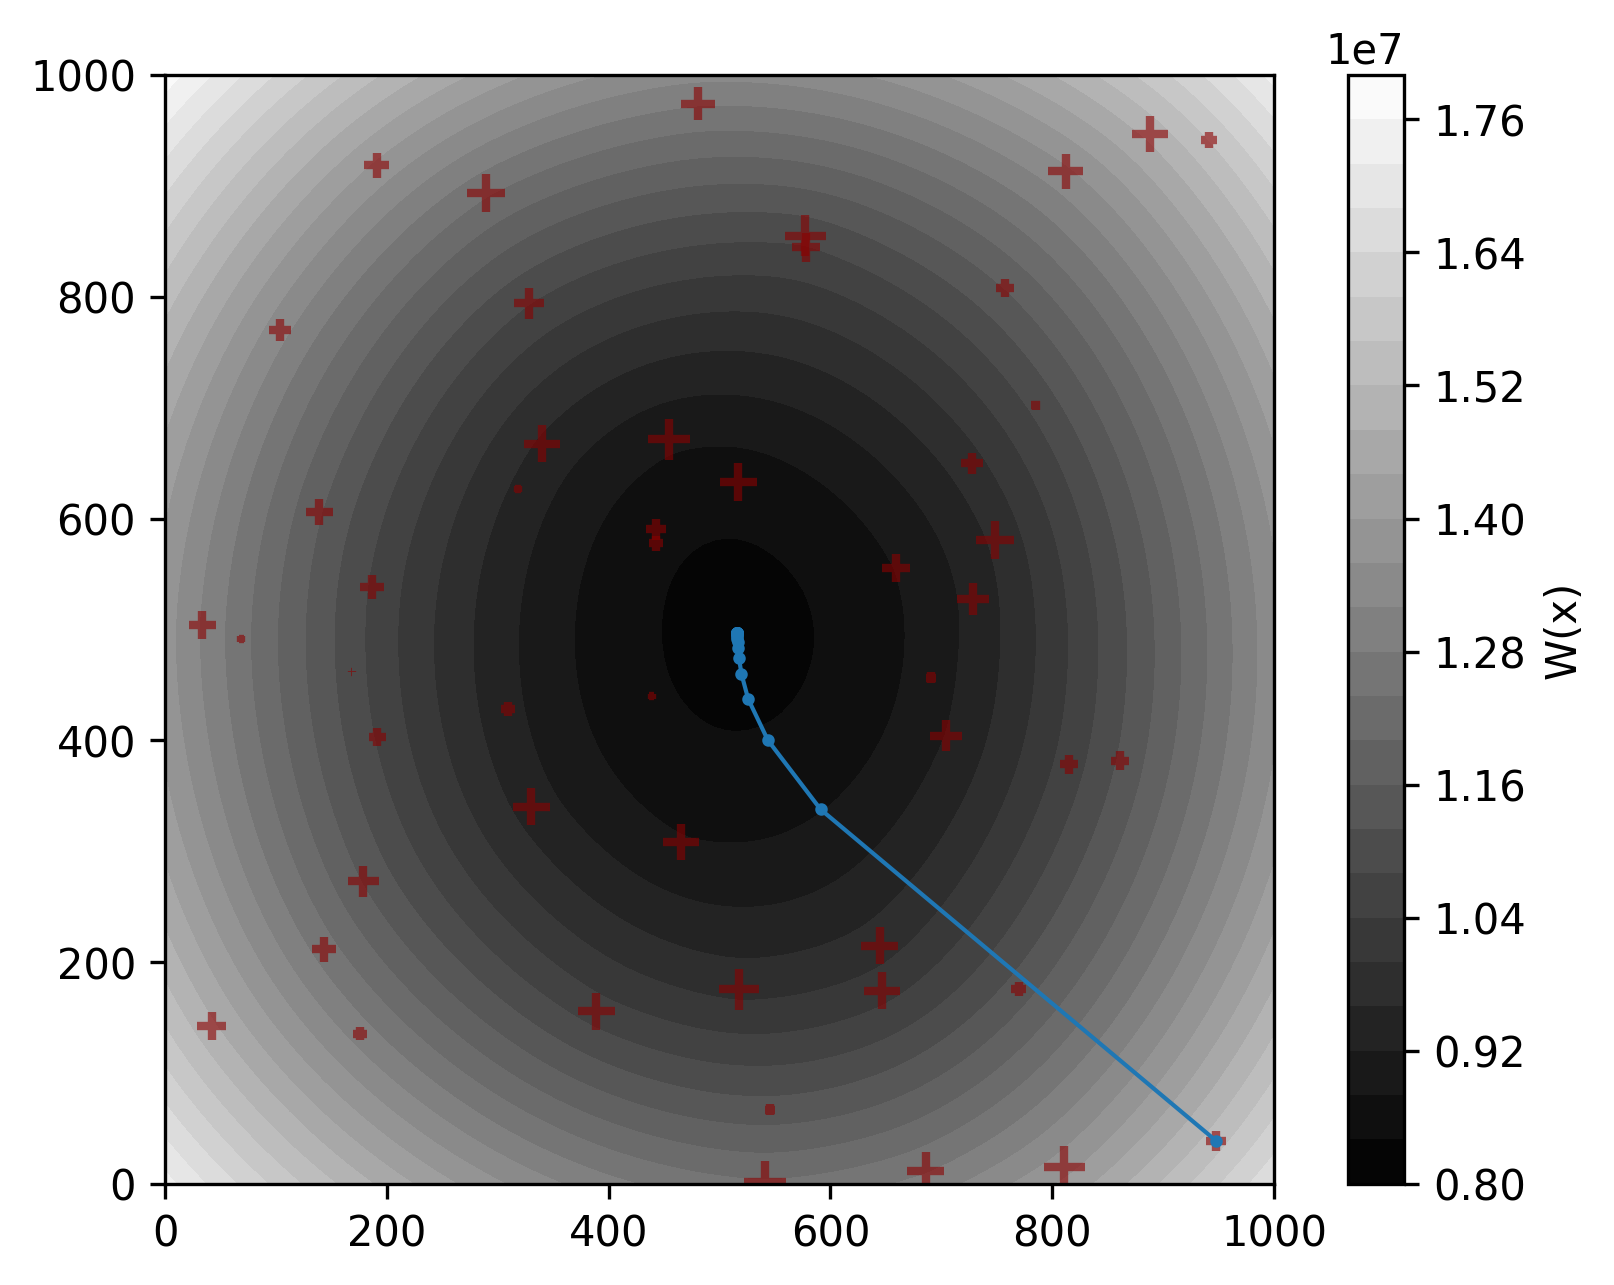
\includegraphics[width=\linewidth]{figuras/recorrido_wz_8.png}
		\caption{Weiszfeld}
	\end{subfigure}
	\hspace{0.005\textwidth}
	\begin{subfigure}[t]{0.4\textwidth}
		\centering
		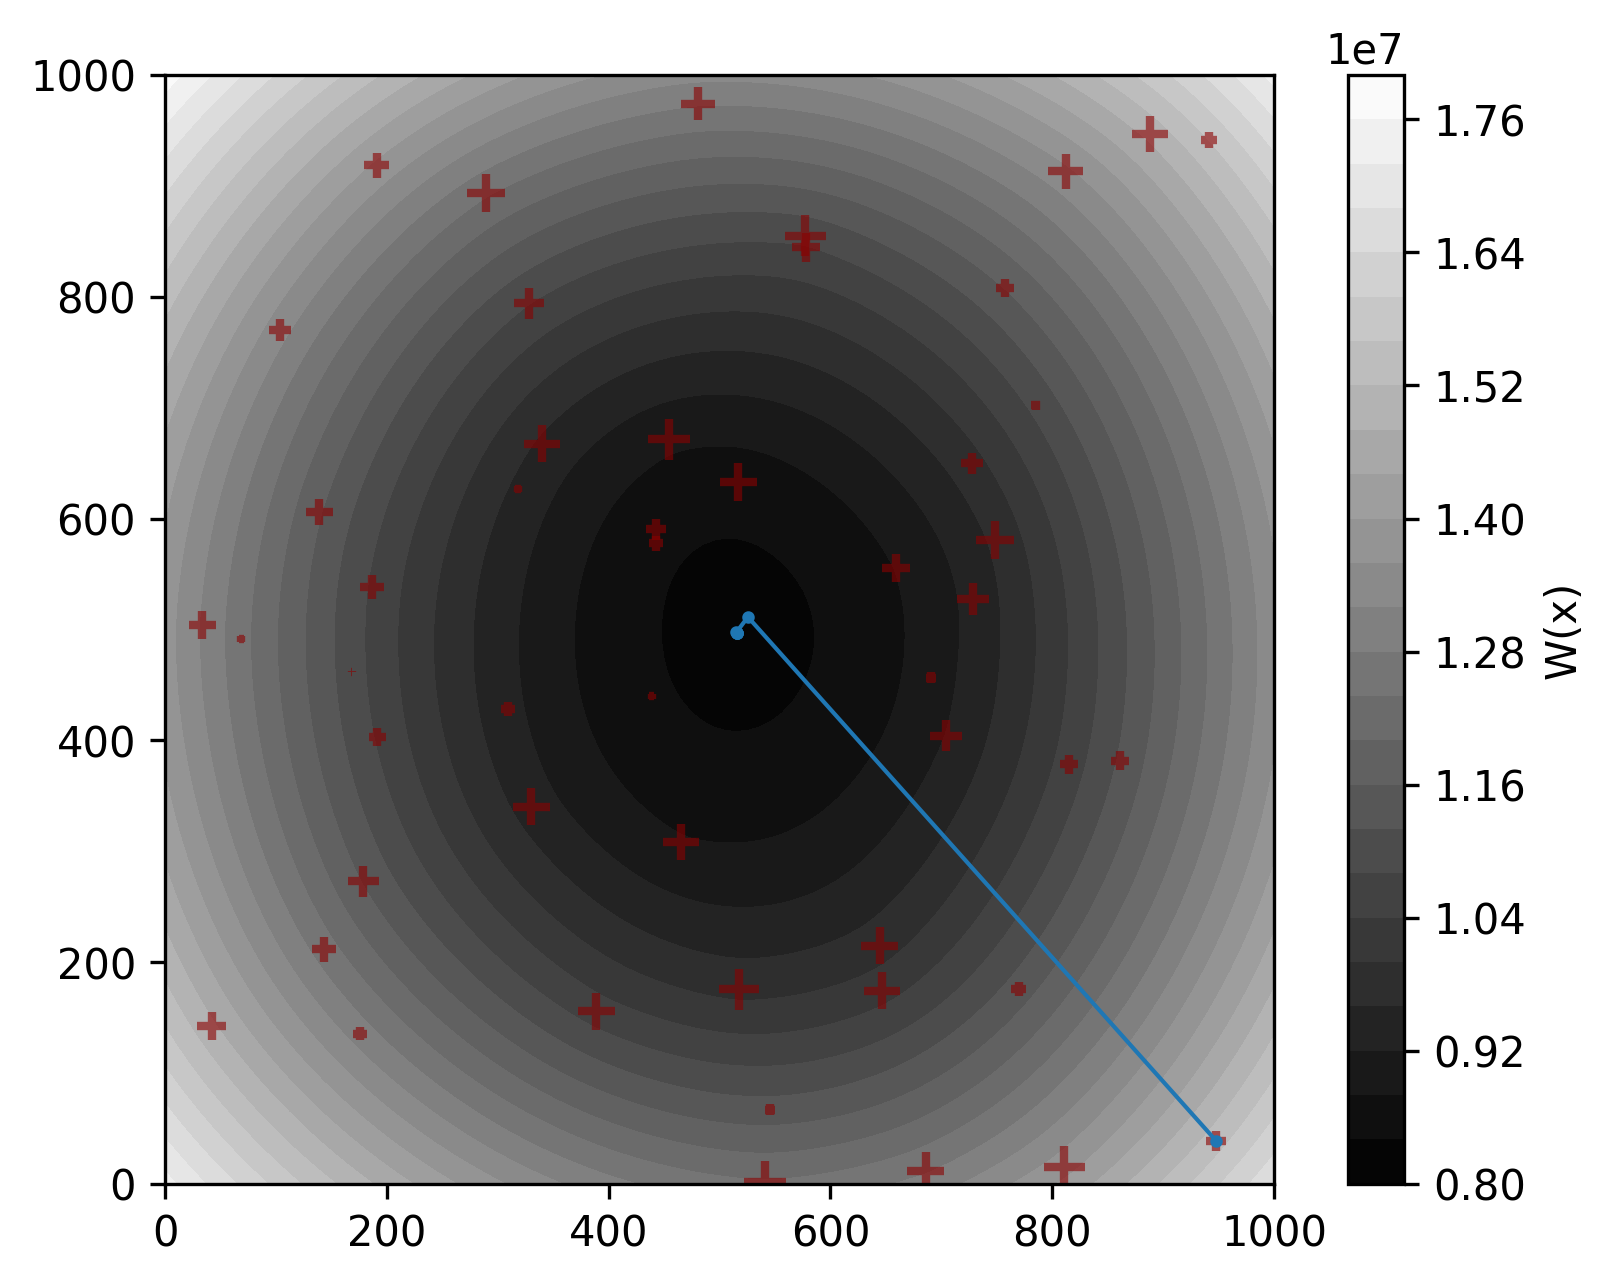
\includegraphics[width=\linewidth]{figuras/recorrido_hj_8.png}
		\caption{Hooke-Jeeves}
	\end{subfigure}
	\hspace{0.005\textwidth}
	\begin{subfigure}[t]{0.4\textwidth}
		\centering
		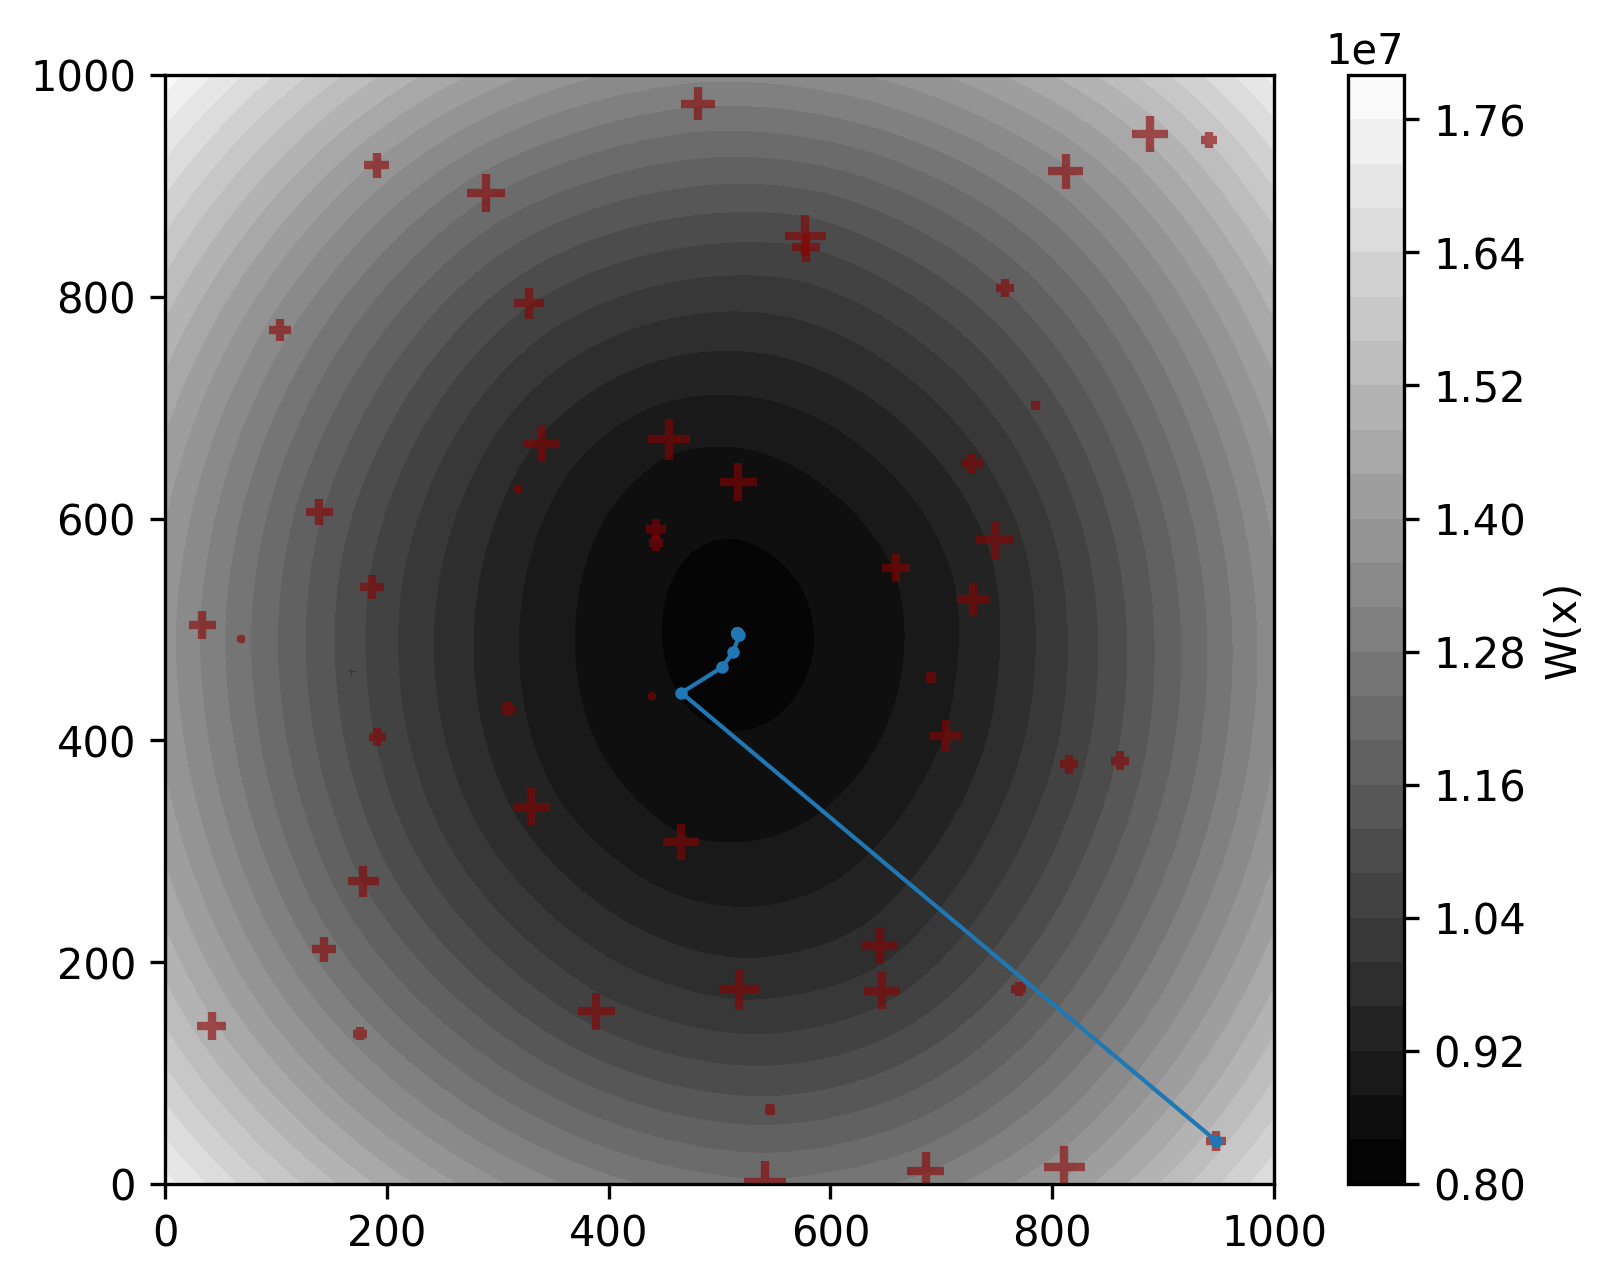
\includegraphics[width=\linewidth]{figuras/recorrido_dg_8.png}
		\caption{Descenso de Gradiente}
	\end{subfigure}
	\caption{Recorridos para los distintos métodos en una misma instancia con 50 puntos ponderados y el contorno de W(x).}
	\label{fig:recorridos_instancia_8}
\end{figure}


Para el análisis implementamos dos tipos de instancias, una con distribución uniforme y otra con clusters definidos que generaban una mayor densidad alrededor de cinco centroides distintos. Para cada tipo generamos cinco replicas de instancias con 100, 500, 1000, 5000 y 10.000 nodos en dos dimensiones distintas, $\mathbb{R}^3$ y $\mathbb{R}^{10}$. Cada instancia se resolvió con los tres algoritmos utilizando un mismo criterio de parada, que la norma de la diferencia entre una iteración y la siguiente sea menor a $10^{-6}$, esto es válido porque la función W que estamos evaluando es convexa, por lo que nos aseguramos estar convergiendo al mínimo global.





\subsection{Conclusión}

\end{document}